\documentclass[11pt]{article}
\usepackage[utf8]{inputenc}
\usepackage[margin=1in]{geometry}
\usepackage{amsmath}
\usepackage{amsfonts}
\usepackage{amssymb}
\usepackage{graphicx}

\title{Feature Selection and Image Classification}
\author{Landon Carter and Courtney Guo}
\date{December 2015}

\begin{document}

\maketitle

\section{Introduction}
In this work, we wish to implement supervised image clustering and classification which combines a feature extraction step with a clustering step. For the feature extraction stage, we will use two different methods: autoencoders and convolutional neural networks. For the clustering stage, we will use softmax layers in the respective neural nets, SVM, and k-means. We will then show the results of these algorithms on the CIFAR-10 image classification dataset.

\section{Feature Selection}
\subsection{Autoencoder}
We used \texttt{MATLAB}'s built in autoencoder implementation on the CIFAR-10 dataset. An autoencoder is a neural network used for learning efficient codings: it is trained such that its output matches its input, but it has a hidden layer in which the number of hidden nodes is less than the number of input nodes. Therefore, the autoencoder will learn to compress the data efficiently, and then decode the data to match the original input. The hidden layer represents the encoding scheme, so we can use the activations of the hidden layer as the features. Training the autoencoder is the same as training a neural network: for each data point we can perform back propagation to calculate the gradients of the error with respect to the weights, and then update the weights based on that, until the error converges or we reach the maximum number of iterations. In particular on the autoencoder, we do not need any labels - we simply try to reconstruct the input. In some implementations, the decoding weights can be inverted from the encoding weights such that the autoencoder is symmetric, though ours were not.

Autoencoders can also be stacked to produce deep neural nets, which can be significantly more effective than one-layer autoencoders, since they can learn higher-order features more easily. One nice feature is that each layer of the deep autoencoder can be trained independently relatively quickly to give approximately-optimal results. The entire deep neural net can then undergo full backpropagation to converge quickly to final optimal values. This method of training is significantly faster than traditional full backpropagation, since each iteration of optimizing a layer is much faster than full backpropagation, and the final full backpropagation step undergoes relatively few iterations since all weights are already close to optimal values.


\subsection{Convolutional Neural Network}
Convolutional neural networks (ConvNet's, or CNN's) are a particular type of neural net which is useful in image analysis and recognition. The distinguishing factor of CNN's are the way they can account for proximity in data, taking ``convolutions'' of small contiguous subsets of the data. This is of particular importance in image processing, where large amounts of information and context can be gained by considering neighboring pixels. The CNN we constructed was based off a standard LeNet topology, consisting of 5 distinct blocks: 3 blocks of convolutional layer, Rectified Linear Unit (ReLU) activation layer, and pooling layer. After these 3 blocks (9 total layers), we had a final 4 layers which computed another convolution, ReLU, convolution, and then softmax in order to do a final bit of convolution before extracting labels. When paired with clustering methods, the output of the final convolution layer was sent to $k$-means and SVM instead of the softmax layer.

After constructing the CNN and initializing it with random values, the CNN is trained via stochastic gradient descent (SGD).

\subsubsection{Convolutional Layer}
The convolution layer is the most important part of the CNN, and is what distinguishes it most distinctly from other neural network topologies. Each convolutional neuron takes some small contiguous subset of the input layer and computes

\[ y_{i''j''d''} = \sum_{i'=1}^{H'}\sum_{j'=1}^{W'}\sum_{d'=1}^{D} f_{i'j'd} \times x_{i''+i'-1,j''+j'-1,d',d''} \]

In other words, for the coordinate $(i'',j'',d'')$, the convolution is determined by applying some filter $f_{i'j'd}$ to each of the inputs within $H',W',D$ of the coordinate of interest (where the original input size is $\mathbf{x} \in \mathbb{R}^{H\times W\times D}$). In this formulation, only inputs to the right and below the desired coordinate are considered (all depth dimensions - usually corresponding to different color channels - are used), though this does not affect the results - the output nominally for coordinate $(i'',j'',d'')$ really corresponds to the output for coordinate $(i''+H'/2,j''+W'/2,d'')$ in the traditional formulation, which considers inputs in the range $H'/2$ to the left, $H'/2$ to the right, and so on. The input is padded with a reasonable value such that edge effects are minimized. This can be demonstrated by considering the 1-dimensional case:
\begin{center}
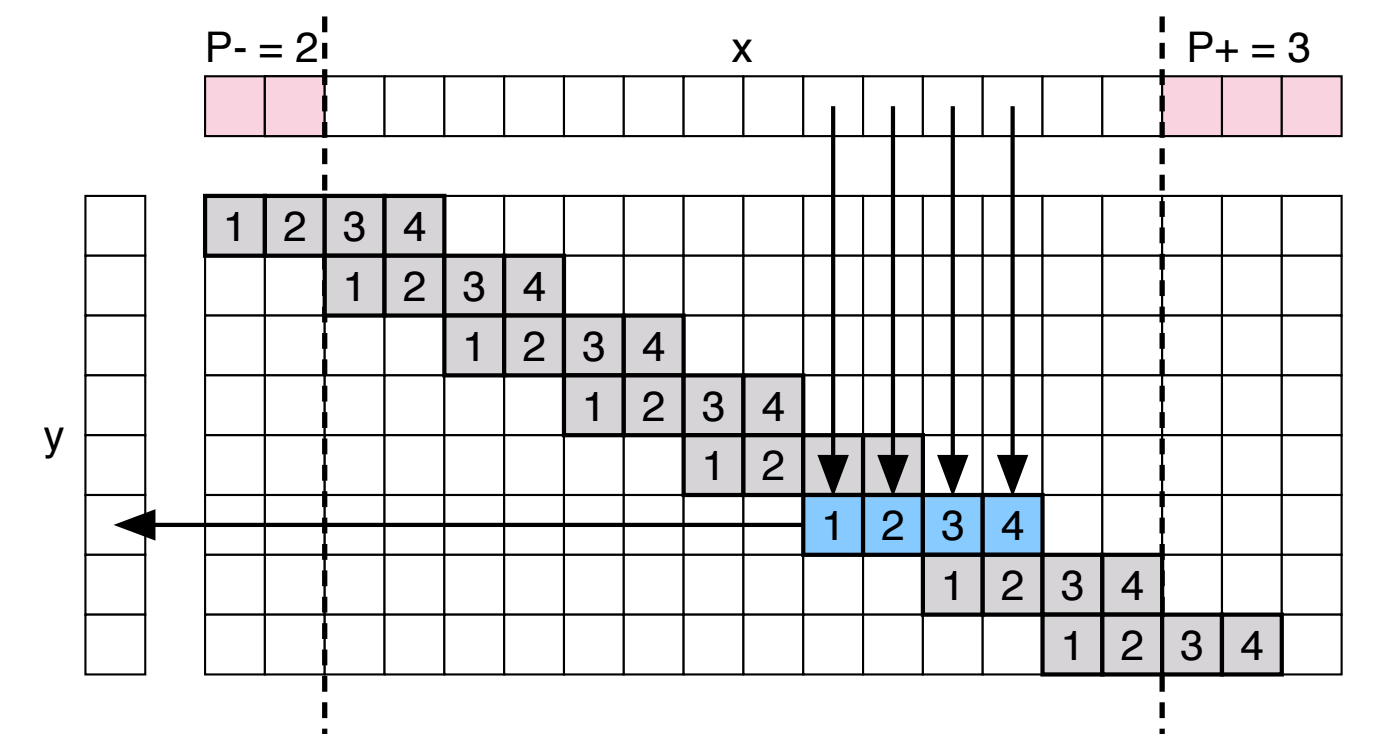
\includegraphics[scale=.5]{convolution.PNG}
\end{center}

Here we can see the operation of a 1-d convolution, with $H' = 4$. Some filter is applied to boxes 1-4 at each $x$, which is then stored in the output $y$. In this case, the padding is made explicit as $P_{-} = 2, P_{+} = 3$.

The filters are equivalent to the weights of normal neural networks, and are initialized randomly within a set of reasonable values. This implementation is relatively fast, because the number of weights is actually independent of input size - there are $d''$ filters defined over an $H'\times W' \times D$ volume, and each filter is applied across the entire input and trained across the entire input. For example, one basic filter may learn edge-detection. One artificial filter that this can be compared to is the Sobel filter, a convolution kernel which represents edge detection in traditional image processing:

\[
G_x =
\begin{bmatrix}
    -1       & 0 & +1 \\
    -2       & 0 & +2 \\
    -1       & 0 & +1
\end{bmatrix},
G_y = 
\begin{bmatrix}
    -1       & -2 & -1 \\
    0       & 0 & 0 \\
    +1       & +2 & +1
\end{bmatrix}
\\,
\mathbf{G} = \sqrt{G_x^2 + G_y^2}
\]

The equivalent convolution filter learned in the CNN might represent just vertical or horizontal edges. With enough filters, many unique image features can be learned. However, as is obvious, the use case of a single convolution layer is very limited, which is why we pair it with a ReLU and pooling layer, and use this trio to construct a deep NN.

\subsubsection{Rectified Linear Unit Layer}
The ReLU layer is a simple activation layer, which computes

\[ y_{ijd} = \max\{0,x_{ijd}\} \]

This performs the same function as any other activation layer - adding nonlinearity to the NN. In this case, a linear activation is selected due to computational speed - it is much faster to compute a linear activation than a sigmoid, while the performance is only minimally decreased.

\subsubsection{Pooling Layer}
The pooling layer computes the maximum input in an $H' \times W'$ patch:

\[ y_{i''j''d} = \max_{1\le i' \le H',1\le j' \le W'} x_{i''+i'-1,j''+j'-1,d} \]

This is useful for selecting the dominant features within each patch and essentially sparsify the data. Importantly, the pooling layer patches are non-overlapping, while the convolutional layers are not. This is also useful for providing robustness to image translation - if an image is translated by less than $H'$ or $W'$, the output of the pooling layer will still be the same.

\subsubsection{Softmax Layer}
The softmax layer is the standard classification layer discussed in class:

\[ y_{ijk} = \dfrac{e^{x_{ijk}}}{\sum_{t=1}^D e^{x_{ijk}}} \]

As discussed in class, this is useful for classification purposes. In other variations we tested, we replaced this layer with $k$-means clustering and multiclass SVM.


\section{Clustering}
\subsection{$k$-means}
$k$-means clustering is an unsupervised learning algorithm that takes a dataset and attempts to group the data into $k$ clusters such that the sum of the distances from each point to the centroid of the cluster that it belongs to is minimized. The algorithm works by first initializing the centroids of $k$ clusters, and at each step, it classifies the points based on which cluster it is closest to, and then updates the centroids of the clusters. One of the benefits of $k$-means clustering is that it will return the coordinates of the centroids of all the clusters, so for each cluster, we have a point that is ``most representative" of the cluster.\\~\\
We implemented the $k$-means algorithm ourselves. We first tested it on the MNIST raw data, which is a database of images of handwritten digits 0-9. Each image is grayscale and is 28 pixels by 28 pixels, and there are 5000 images in the dataset. So each data point can be represented as a feature vector of size $28^2 = 784$. We ran our $k$-means implementation on the MNIST dataset with $k=10$, and initial centroids set equal to 10 random data points. To assign classes to clusters, for each cluster we looked at the label with the majority vote in each cluster, and assigned that label to that cluster. Therefore, to classify a new point, we first find out which cluster it is closest to, and then assign it the label corresponding to that cluster. To measure performance of the $k$-means clustering, we counted the number of misclassified points in the test set. For the MNIST dataset, we got an error rate of $\frac{3695}{5000} = 73.9\%$, suggesting that $k$-means does not work well on this dataset. However, it is slightly better than random, because a random classifier would give a $90\%$ error rate. However, once we consider the 5 most likely labels for each data point, we have a $21.2\%$ error rate, so our classifier is nontrivially better than random. We compared our implementation with MATLAB's built-in $k$-means algorithm and they got almost identical results, so it is not a problem with our implementation. \\~\\
We thought one possible reason $k$-means doesn't work well might be because the dimensionality is too high, so we used an autoencoder to reduce the 784 features to 50, and then used $k$-means on the 50 features. However, we still got a high error rate of $\frac{3570}{5000} = 71.4\%$. Therefore, this suggests that the MNIST data is not suited for $k$-means. Possible reasons for this might be because there is a lot of overlap between clusters, so $k$-means cannot distinguish between them well. One other possible reason for poor performance is the highly correlated dependence between various dimensions, such that applying a kernel or a neural network to them will separate the clusters much better.

\subsection{Support Vector Machine}
Support Vector Machines are supervised learning models that construct a hyperplane to separate the dataset, classifying all points on one side of the hyperplane as belonging to one class, and all points on the other side as belonging to the other class. SVM aims to maximize the margin of the classification, which is the distance from the closest training point to the hyperplane. Finding the hyperplane with maximum margin can be expressed as a quadratic optimization problem (minimizing an objective while satisfying some constraints), so we can take the dual form as shown in homework 2 to solve the optimization problem. SVM is a binary classifier, so to extend it to $n$ classes, we can train $n$ one-vs-all classifiers: the $i^{\text{th}}$ classifier's output represents whether or not the point is in the $i^{\text{th}}$ class. We adapted our code from homework 2 to extend it to the multiclass case by training one-vs-all classifiers. However, the code ran too slowly for our purposes, so we used an existing implementation of SVM along with our same multiclass extension.

\section{Results}
The CIFAR-10 dataset consists of images corresponding to 10 different classes: airplane, automobile, bird, cat, deer, dog, frog, horse, ship, and truck. Each image is a $32 \times 32$ color image, and there are 10000 examples in the training dataset, and 10000 examples in the test dataset. We can find the results of each combination of feature selection and clustering on the CIFAR-10 dataset.

\subsection{Autoencoder}
\subsubsection{Autoencoder with softmax}
We added a softmax layer to the autoencoder, so that the diagram of the neural network is given below:
\begin{center}
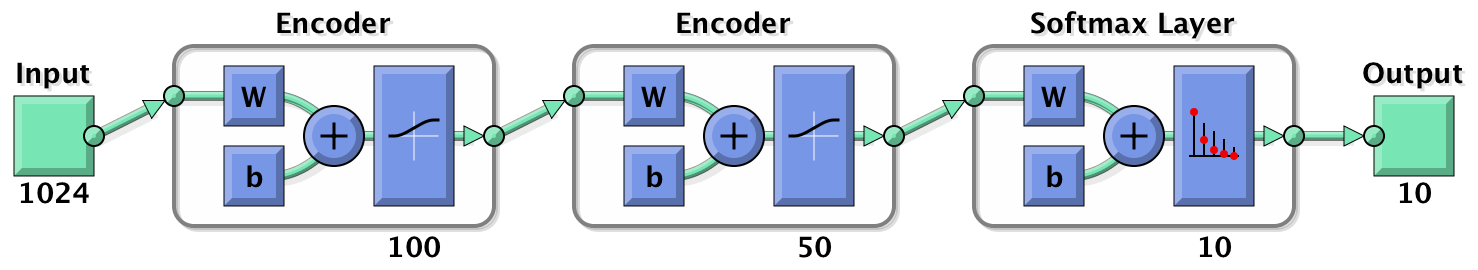
\includegraphics[scale=0.6]{autoencoder.png} \\
\end{center}
We can also plot the weights of the first layer of the autoencoder, to see what kind of features it learned. We see that there is a little overfitting, because some of the nodes clearly resemble some of the original pictures, but otherwise it seems like the autoencoder has learned some important features.
\begin{center}
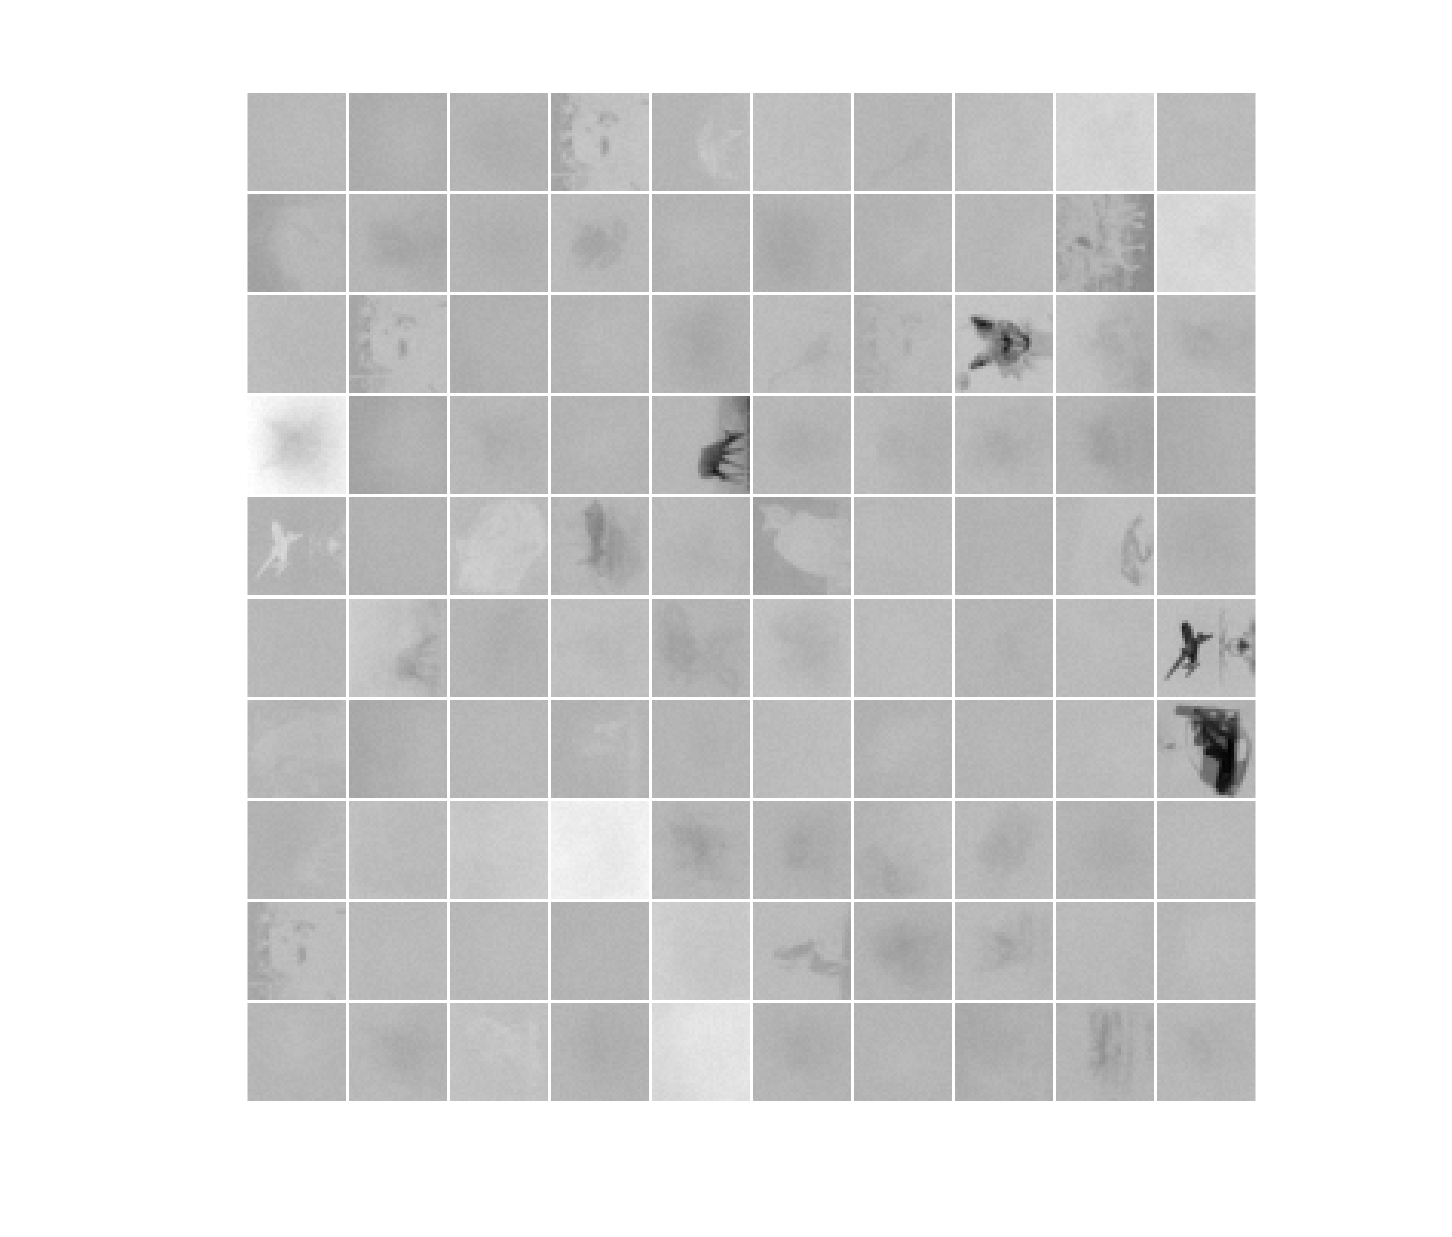
\includegraphics[scale=0.3,angle=270]{cifar-10-layer1weights.png} \\
\end{center}
Then, we can plot the confusion matrix, which shows how similar our classification is to the true labels of the data. This plot shows all of the counts for which a data point was classified by our classifier as belonging to class $i$, but it actually belongs to class $j$. Therefore the entries on the diagonal are when $i=j$, which are the cases when our classifier was correct. We see that our accuracy was 34\% (therefore error rate was 66\%), which is significantly better than random, but it is not very good.
\begin{center}
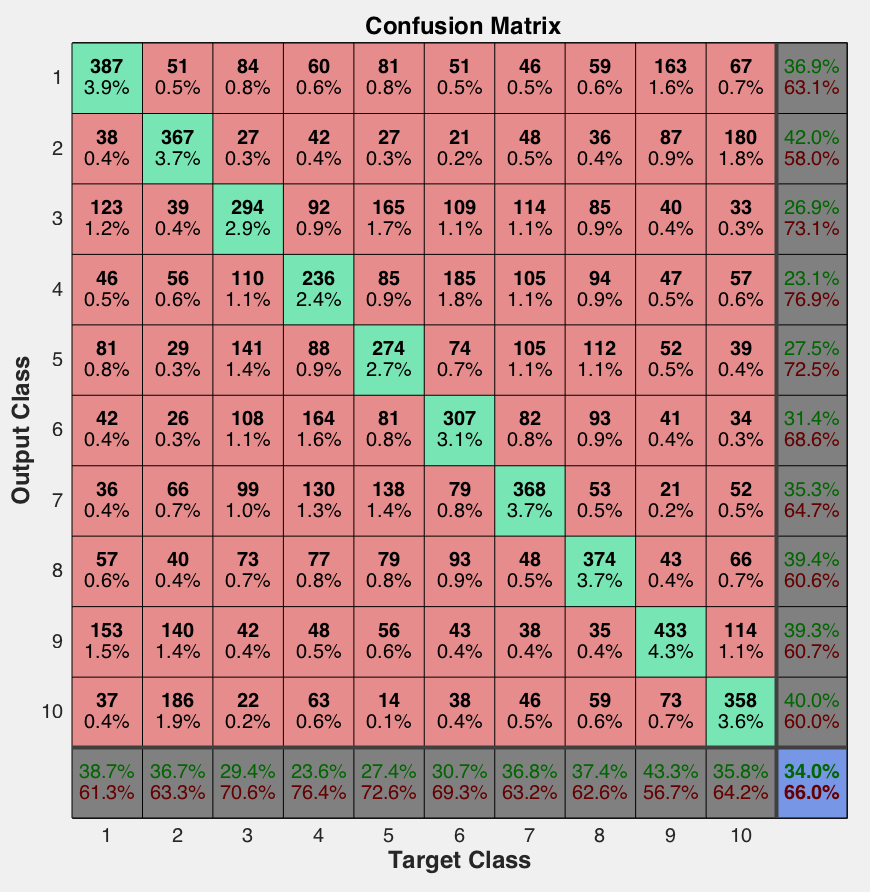
\includegraphics[scale=0.5]{confusion.png} \\
\end{center}

\subsubsection{Autoencoder with SVM}
We used the features extracted by the autoencoder as inputs to the one-vs-all SVM multiclass method. On the CIFAR-10 dataset, all of the one-vs-all classifiers outputted 0 for all the data points, so none of the points were actually classified. This meant that none of the classes were significantly likely. Since we could not get any results for the CIFAR-10 dataset, we tried this method on the MNIST dataset. Around half of the data points were not classified by any of the 10 SVM classifiers, but some of the data points were classified, and the accuracy was high for those cases. If a data point was not classified by any of the 10 SVM classifiers, it gets assigned the 10th class by default.
\begin{center}
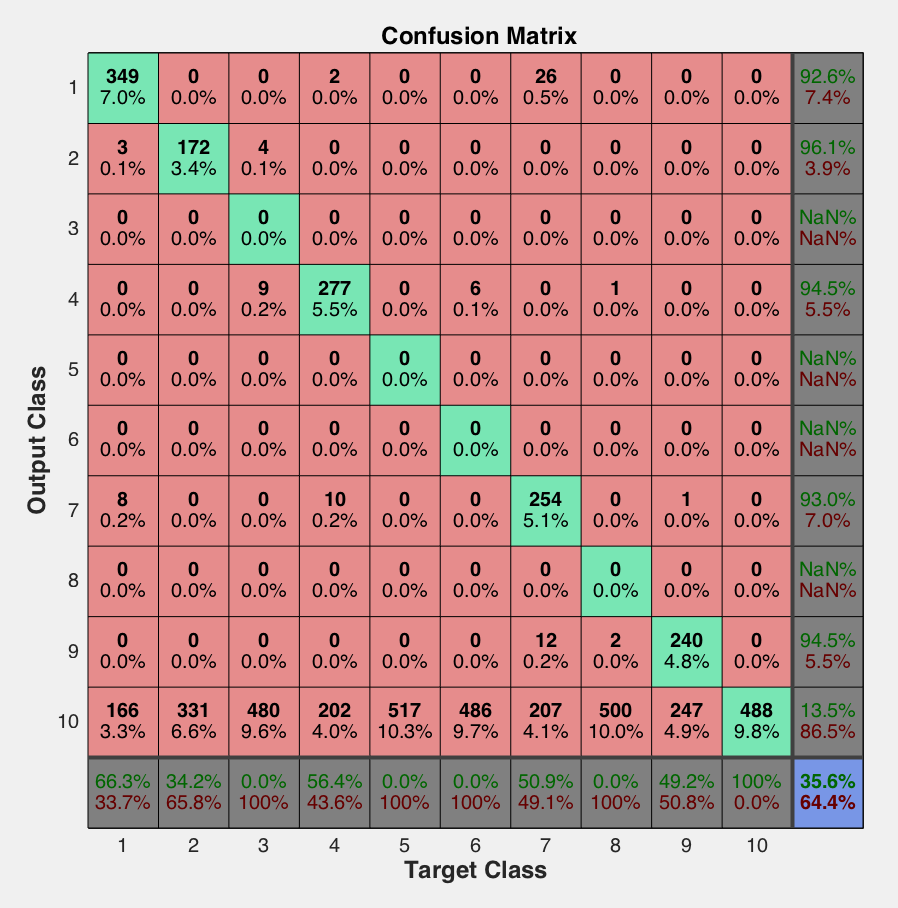
\includegraphics[scale=0.5]{autoencoder_svm_mnist.png}
\end{center}
This plot is a confusion matrix, explained earlier. We can see that our classifier only predicted classes of 1, 2, 4, 7, 9, and 10. When it did not predict 10, its accuracy was 93.9\%, which is pretty remarkable, but it predicted 10 most of the time which meant that the classifier was unsure on most of the data points. Therefore, we see that the one-vs-all strategy for multiclass SVM does not yield the best results, because if there is no class is more than 50\% likely for a given point, SVM will not classify the point into any class.

\subsubsection{Autoencoder with $k$-means}
We ran the $k$-means algorithm on features extracted using an autoencoder, but the algorithm converged to only have one cluster. This probably means that the features extracted were not distinct enough, so the $k$-means algorithm could not find two separate clusters that would be more optimal than one cluster. From the confusion matrix below, we see that the accuracy of this is 10.3\%, which is basically equivalent to random guessing. From our discussion of $k$-means above, this low accuracy is expected, because $k$-means did not work well with MNIST, and classification on the CIFAR-10 dataset is harder than classification on MNIST.
\begin{center}
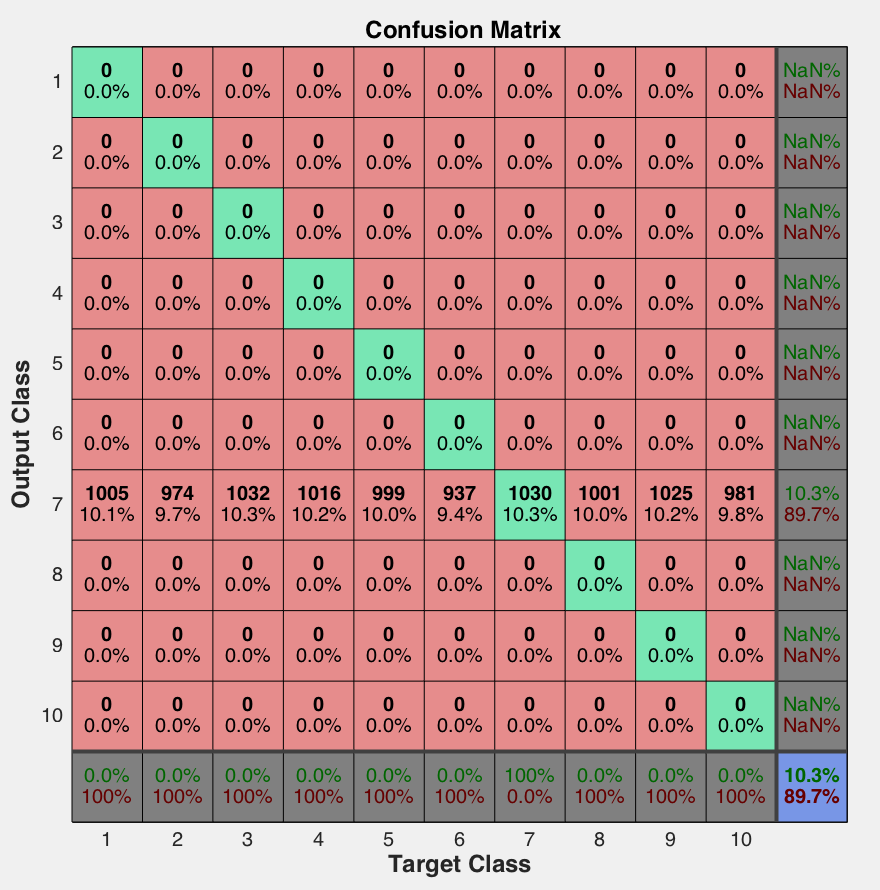
\includegraphics[scale=0.5]{autoencoder_kmeans.png}
\end{center}

\subsection{Convolutional Neural Network}
\subsubsection{Convolutional Neural Network with Softmax}

The training of the CNN proceeded via SGD as mentioned, attempting to minimize an energy function which essentially captured the error in training. The error and objective function for the training data and validation data was plotted over the course of 30 epochs of training. After about 15 epochs, it can be seen that the validation error rate has stabilized to around 20\%. When including the top 5 results of the CNN, validation error rate stabilized to less than 3\% (\texttt{valtop5e}). In this case, each epoch represents passing through the entire training set, or 10,000 individual SGD steps.

\begin{center}
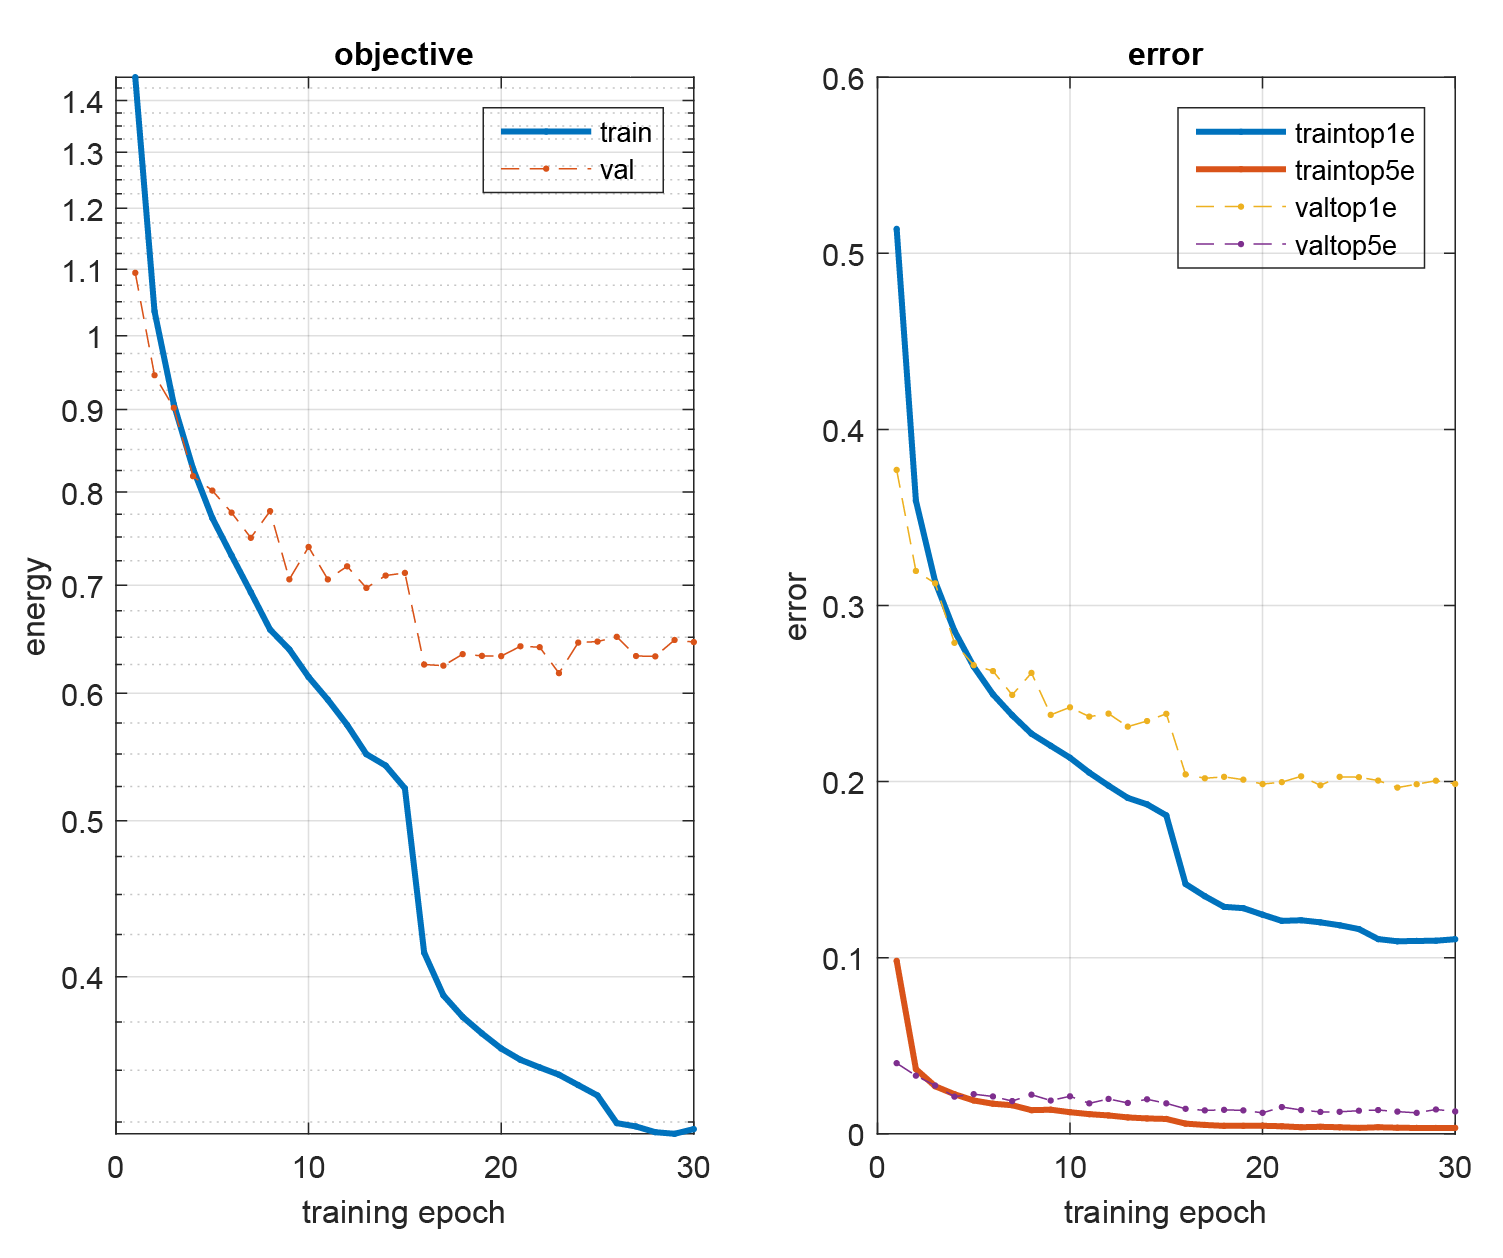
\includegraphics[scale=0.35]{convnet_train.PNG} \\
\end{center}

This final error of around 20\% is notable, since it is in the same ballpark as the best results obtained for CIFAR-10, which report as low as 15\% error without data augmentation (we also don't use data augmentation, so this is a valid comparison). This was achieved with a very similar structure to the CNN - softmax combo we used to classify CIFAR-10, but with optimized weights for hyperparameters such as learning rate. The same approximate structure is found in GoogLeNet, which won the most recent ImageNet classification challenge.

\subsubsection{Convolutional Neural Network with SVM}

Multiclasss SVM was much more successful in clustering the feature vectors from CNN's than autoencoders, reaching a final accuracy of a very disappointing 11.5\% (hardly better than random guessing). Again, label 10 was assigned by default if no other label had probability >50\%. Interestingly, labels 3 and 9 seemed popular for the SVM to predict, though it is unclear why this might be the case, and merits future analysis.

\begin{center}
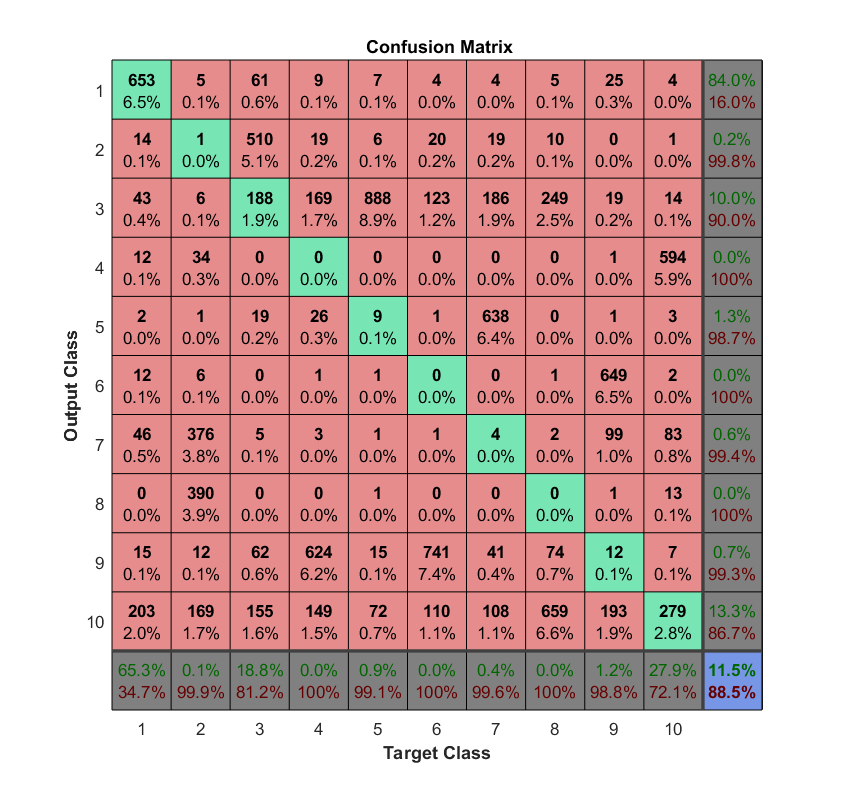
\includegraphics[scale=0.4]{convnet_svm_3.png}
\end{center}

\subsubsection{Convolutional Neural Network with $k$-means}

By taking the activations of the last convolution layer, right before the softmax layer, we obtain a lower-dimensionality representation of our input. Rather than send this to softmax, we instead used this as the input data for $k$-means clustering, where again the most common label within each cluster was assigned to the cluster. This yielded quite decent results, with an overall 63.9\% accuracy, significantly better than any other feature extraction/classification pair except CNN with softmax, which achieved an 80\% overall accuracy.
\begin{center}
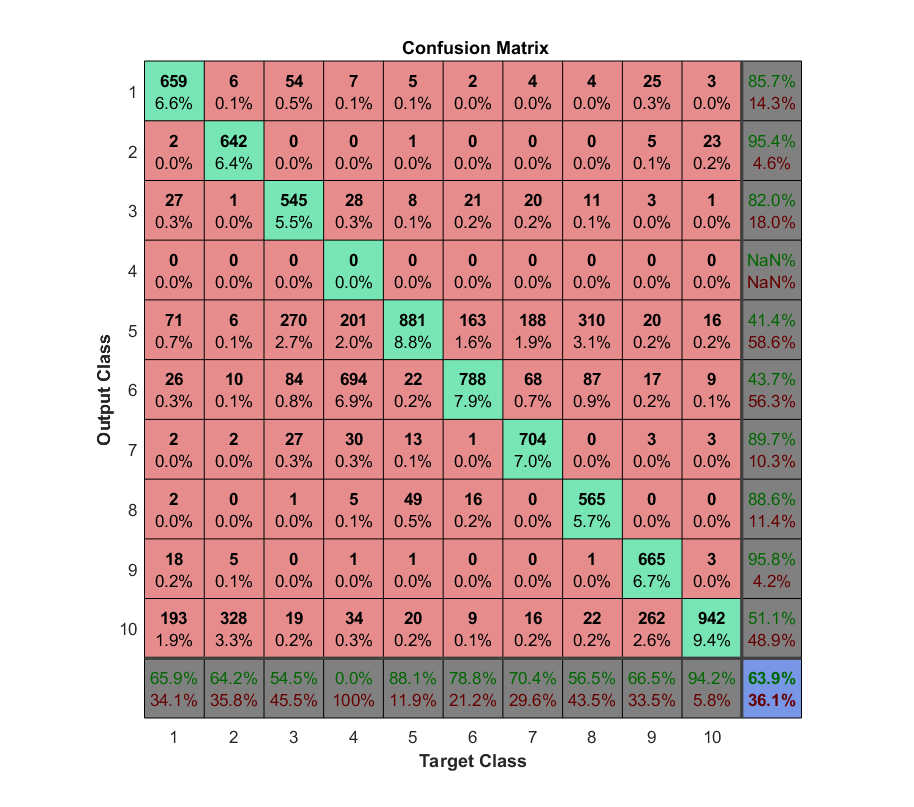
\includegraphics[scale=0.4]{convnet_kmeans.png}
\end{center}


\section{Discussion}
Convolutional Neural Networks with a softmax classifier were by far the most effective pairing of feature extraction and classification. This makes sense - they're the state of the art for image classification, due to convolutional neural networks' ability to efficiently extract contextual image information and softmax's kernel-like trainability. It is understandable that the more optimized topology of the CNN would easily surpass the accuracy of the autoencoder.

Most interestingly, taking the final 64-dimensional activations of the final convolutional layer in the CNN and using them as inputs to a $k$-means clustering algorithm yielded very favorable results, achieving a very respectible 64\% accuracy on CIFAR-10. This also holds potential interest, since $k$-means is an unsupervised clustering algorithm, it could theoretically be used in a semi-supervised classification task, where it would know to create a separate cluster for previously-unseen data. The effectiveness of this strategy is tremendously amplified when feeding it outputs from a CNN than raw data, and clustering can be done much more quickly due to the significantly decreased dimensionality. In order to be able to tell when a new cluster is added, a regularization function on the number of clusters would have to be introduced and the number of clusters allowed to vary.

Overall, the strategy of coupling a simple clustering algorithm to a feature extraction algorithm was less successful than anticipated, most likely due to the very high covariance of the extracted features, which prevents standard non-kernelized clustering algorithms from performing well. Manually kernelizing a clustring algorithm was not pursued due to the difficulty in coming up with a reasonable kernel for the artificial data. Softmax instead served as a substitute, allowing something similar to a kernelized clustering algorithm to be learned by the NN's.

\section{Works Cited}
\begin{itemize}
\item Learning Multiple Layers of Features from Tiny Images, Alex Krizhevsky, 2009.
\item ``MatConvNet - Convolutional Neural Networks for MATLAB'', A. Vedaldi and K. Lenc, Proc. of the ACM Int. Conf. on Multimedia, 2015.
\end{itemize}
\end{document}
-